\section{Planetas}
	\subsection{Descripción del problema}
	Se desarrollo un programa para observar en que momento falla el tener $n$ numero de elementos en 3 grupos, se le llama fallar al punto en el que solo hay elementos en uno de los grupos.
	El procedimiento se realiza tomando 1 elemento de dos de los grupos y así obtener 2 nuevos elementos en el otro conjunto como en la figura \ref{fig:marcianos}.
	\begin{figure}[H]
		\begin{center}
			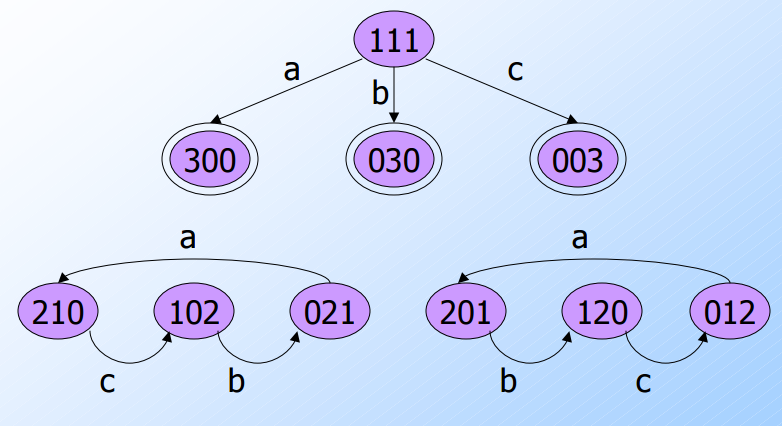
\includegraphics[width=10cm, height=4cm]{img/marcianos.png}
			\caption{Ejemplo de funcionamiento con 3 elementos.\cite{WEB}}
			\label{fig:marcianos}
		\end{center}
	\end{figure}
	Se mostraran los diferentes caminos que puede tomar el proceso al introducir el numero de los elementos. El programa cuenta con modo manual y automático.
	\subsection{Código}
	El código fue realizado en C.
	\\Archivo: arbol.h
	\begin{lstlisting}[language=C]
	#ifndef __ARBOL__
	#define __ARBOL__

	#include <stdio.h>
	#include <stdlib.h>

	struct Nodos{
	  int dato[3];
	  struct Nodos *siguiente;
	};

	typedef struct Nodos Nodo;

	struct Arbol{
	  int elemento[3];
	  struct Arbol *arbolA;
	  struct Arbol *arbolB;
	  struct Arbol *arbolC;
	  Nodo *primero;
	};
	int insertar(struct Arbol **, int[3], Nodo *, int);
	int crear_arbol(struct Arbol **, int[3], Nodo *);
	void imprimir_arbol(struct Arbol *, int);

	#endif
	\end{lstlisting}
	Archivo: arbol.c
	\begin{lstlisting}[language=C]
		#include "arbol.h"
		int insertar(struct Arbol **arbol, int valor[3], Nodo *lista, int continuar) {
		    int valor_aux[3];
		    struct Arbol *arbol_nuevo = NULL;
		    if(arbol == NULL) {
		        return -1; //No existe
		    }
		    int existe_arbol_nuevo = crear_arbol(&arbol_nuevo, valor, lista);
		    if(existe_arbol_nuevo==-1) {
		        return -1; // No existe
		    }
		    if (*arbol == NULL) {
		        *arbol = arbol_nuevo; //Raiz
		    }
		    if (continuar == 0){
		        return 1;
		    }
		    if (valor[1] > 0 && valor[2] > 0) {
		        int repetido =0;
		        valor_aux[1] = valor[1] - 1;
		        valor_aux[2] = valor[2] - 1;
		        valor_aux[0] = valor[0] + 2;
		        Nodo *mas = arbol_nuevo->primero;
		        while(mas != NULL){
		            if((mas->dato[0] == valor_aux[0])&&(mas->dato[1] == valor_aux[1])&&(mas->dato[2] == valor_aux[2])) {
		                repetido = 1;
		                break;
		            }
		            mas = mas->siguiente;
		        }
		        if (repetido == 0){
		            insertar(&((*arbol)->arbolA), valor_aux, arbol_nuevo->primero, 1);
		        } else{
		            insertar(&((*arbol)->arbolA), valor_aux, arbol_nuevo->primero, 0);
		        }
		    }
		    if (valor[0] > 0 && valor[2] > 0) {
		        int repetido =0;
		        valor_aux[0] = valor[0] - 1;
		        valor_aux[2] = valor[2] - 1;
		        valor_aux[1] = valor[1] + 2;
		        Nodo *mas = arbol_nuevo->primero;
		        while(mas != NULL){
		            if((mas->dato[0] == valor_aux[0])&&(mas->dato[1] == valor_aux[1])&&(mas->dato[2] == valor_aux[2])) {
		                repetido = 1;
		                break;
		            }
		            mas = mas->siguiente;
		        }
		        if (repetido == 0){
		            insertar(&((*arbol)->arbolB), valor_aux, arbol_nuevo->primero, 1);
		        } else{
		            insertar(&((*arbol)->arbolB), valor_aux, arbol_nuevo->primero, 0);
		        }
		    }
		    if (valor[0] > 0 && valor[1] > 0) {
		        int repetido =0;
		        valor_aux[0] = valor[0] - 1;
		        valor_aux[1] = valor[1] - 1;
		        valor_aux[2] = valor[2] + 2;
		        Nodo *mas = arbol_nuevo->primero;
		        while(mas != NULL){
		            if((mas->dato[0] == valor_aux[0])&&(mas->dato[1] == valor_aux[1])&&(mas->dato[2] == valor_aux[2])) {
		                repetido = 1;
		                break;
		            } else{
		            }
		            mas = mas->siguiente;
		        }
		        if (repetido == 0){
		            insertar(&((*arbol)->arbolC), valor_aux, arbol_nuevo->primero, 1);
		        } else{
		            insertar(&((*arbol)->arbolC), valor_aux, arbol_nuevo->primero, 0);
		        }

		    }
		    return 1;
		}

		int crear_arbol(struct Arbol **nuevo, int valor[3], Nodo *lista) {
		    struct Arbol *auxiliar = NULL;
		    auxiliar = (struct Arbol*)malloc(sizeof(struct Arbol));
		    if (auxiliar == NULL) {
		        return -1;
		    }
		    auxiliar->arbolA = NULL;
		    auxiliar->arbolB = NULL;
		    auxiliar->arbolC = NULL;
		    auxiliar->elemento[0] = valor[0];
		    auxiliar->elemento[1] = valor[1];
		    auxiliar->elemento[2] = valor[2];
		    auxiliar->primero = NULL;

		    while(lista != NULL){
		        Nodo **final_lista = &(auxiliar->primero);
		        while(*final_lista != NULL){
		            final_lista = &((*final_lista)->siguiente);
		        }

		        Nodo *temporal = NULL;
		        temporal = (Nodo *) malloc(sizeof(Nodo));
		        if (temporal == NULL){
		            printf("Temporal es null");
		        }
		        temporal->dato[0] = lista->dato[0];
		        temporal->dato[1] = lista->dato[1];
		        temporal->dato[2] = lista->dato[2];
		        temporal->siguiente = NULL;

		        *final_lista = temporal;
		        lista = lista->siguiente;
		    }

		    Nodo **final = &(auxiliar->primero);
		    while(*final != NULL){
		        final = &((*final)->siguiente);
		    }

		    Nodo *temporal = NULL;
		    temporal = (Nodo *) malloc(sizeof(Nodo));
		    if (temporal == NULL){
		        printf("Temporal es null");
		    }
		    temporal->dato[0] = valor[0];
		    temporal->dato[1] = valor[1];
		    temporal->dato[2] = valor[2];
		    temporal->siguiente = NULL;

		    *final = temporal;
		    *nuevo = auxiliar;
		    return 1;
		}
		void imprimir_arbol(struct Arbol *arbol, int n){
		    int contador = 0;
		    if(arbol->arbolA != NULL){
		        imprimir_arbol(arbol->arbolA, n);
		    } else {
		        contador = contador +1;
		    }

		    if(arbol->arbolB != NULL){
		        imprimir_arbol(arbol->arbolB, n);
		    } else {
		        contador = contador +1;
		    }
		    if(arbol->arbolC != NULL){
		        imprimir_arbol(arbol->arbolC, n);
		    } else {
		        contador = contador +1;
		    }
		    if (contador == 3){
		        FILE *archivo = NULL;
		        archivo = fopen("resultado.txt", "a");
		        Nodo *mi_nodo = arbol->primero;
		        while(mi_nodo !=NULL){
		            fprintf(archivo, "[%d,", mi_nodo->dato[0]);
		            fprintf(archivo, "%d,", mi_nodo->dato[1]);
		            fprintf(archivo, "%d]", mi_nodo->dato[2]);
		            fputc(' ', archivo);
		            if(mi_nodo->siguiente ==NULL){
		                if(mi_nodo->dato[0] == n || mi_nodo->dato[1] == n || mi_nodo->dato[2] == n){
		                    fputs("--Falla-- ", archivo);
		                }
		            }
		            mi_nodo = mi_nodo->siguiente;
		        }
		        fputs("\n", archivo);
		        fclose(archivo);
		    }

		}
	\end{lstlisting}
	Archivo: main\_planetas.c
	\begin{lstlisting}[language=C]
		#include <stdio.h>
		#include <stdlib.h>
		#include <time.h>
		#include "arbol.h"
		int menu() {
		    int opcion;
		    printf("Que quieres hacer?\n1.-Manual\n2.-Automatico\n3.-Salir\n");
		    scanf(" %d", &opcion);
		    return opcion;
		}

		int menu_continuar() {
		    int opcion;
		    printf("Intentar otra vez?\nSi = 1 NO = 0\n");
		    scanf(" %d", &opcion);
		    return opcion;
		}

		int random_longitud() {
		    int longitud = 1 + rand() % (1000 + 1 - 1);
		    return longitud;
		}

		void iniciar(int n){
		    FILE *archivo = NULL;
		    archivo = fopen("resultado.txt", "w");
		    fprintf(archivo, "El numero de elementos es:%d \n", n);
		    fclose(archivo);
		    srand(time(NULL));

		    int a = 0;
		    int b = 0;
		    int c = 0;

		    while(1){
		        a = n-b;
		        while(1){
		            int numero[3];
		            struct Arbol *arbol_prueba = NULL;
		            Nodo *lista = NULL;
		            archivo = fopen("resultado.txt", "a");
		            numero[0] = a;
		            numero[1] = b;
		            numero[2] = c;
		            insertar(&arbol_prueba, numero, lista, 1);
		            fputs("Combinacion: ", archivo);
		            fprintf(archivo, "[%d,", numero[0]);
		            fprintf(archivo, "%d,", numero[1]);
		            fprintf(archivo, "%d]\n", numero[2]);
		            fclose(archivo);
		            imprimir_arbol(arbol_prueba, n);
		            a = a-1;
		            c = c+1;
		            if (a<0){
		                break;
		            }
		        }
		        b = b+1;
		        c = 0;
		        if (b == n+1){
		            break;
		        }
		    }
		}

		int main(int argc, char const *argv[]) {
		    int continuar = 1;
		    int manual = 1;
		    int longitud = 0;
		    while(continuar) {
		        manual = menu();
		        if (manual == 1) {
		            printf("%s\n", "Ingresa el numero de elementos  en el intervalo [0-1000]: ");
		            scanf("%d", &longitud);
		        } else if (manual == 2) {
		            longitud = random_longitud();
		        } else {
		            break;
		        }
		        printf("El numero de elementos es: %d\n", longitud);
		        iniciar(longitud);
		        printf("Proceso terminado, revisar archivo resultado.txt\n");
		        continuar = menu_continuar();
		    }
		    return 0;
		}

	\end{lstlisting}
	\subsection{Pruebas}
	Pruebas de las opciones del menú.
	\\
	{\large Modo de manual.}
	\begin{figure}[H]
		\begin{center}
			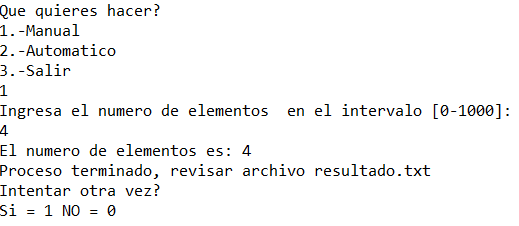
\includegraphics[width=10cm, height=5cm]{img/marcianos-manual-consola.png}
			\caption{Ejecución del programa en modo manual.}
			\label{fig:marcianos1}
		\end{center}
	\end{figure}
	\begin{figure}[H]
		\begin{center}
			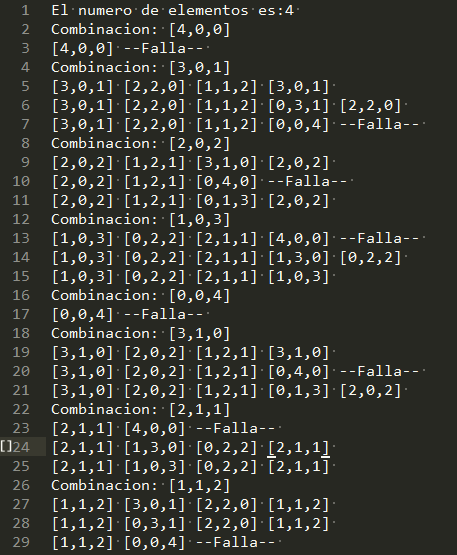
\includegraphics[width=9cm, height=10cm]{img/marcianos-manual-archivo1.png}
			\caption{Resultado del proceso parte 1.}
			\label{fig:marcianos2a}
		\end{center}
	\end{figure}
\begin{figure}[H]
	\begin{center}
		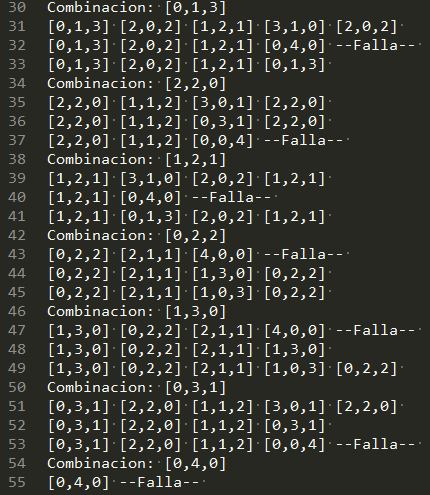
\includegraphics[width=9cm, height=10cm]{img/marcianos-manual-archivo2.png}
		\caption{Resultado del proceso parte 2.}
		\label{fig:marcianos2b}
	\end{center}
\end{figure}
	{\large Modo automático}
	\begin{figure}[H]
		\begin{center}
			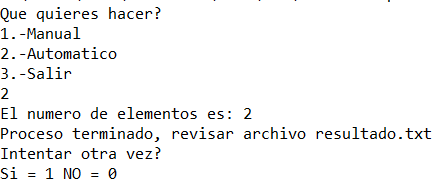
\includegraphics[width=\linewidth, height=7cm]{img/marcianos-automatico-consola.png}
			\caption{Probando el modo automático}
			\label{fig:marcianos3}
		\end{center}
	\end{figure}
	\begin{figure}[H]
		\begin{center}
			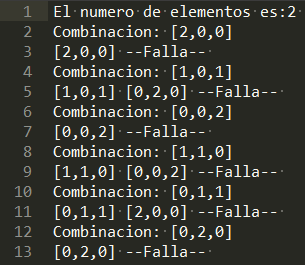
\includegraphics[width=8cm, height=7cm]{img/marcianos-automatico-archivo.png}
			\caption{Resultado de la prueba}
			\label{fig:marcianos4}
		\end{center}
	\end{figure}
